\section{Utilizations of the re module}
\label{sec:utilizations}

\noindent \textbf{Utilization}: A \emph{utilization} occurs whenever a regex appears in source code.  We detect utilizations by statically analyzing source code and recording calls to the {\tt re} module in Python.
Within a source code file, a {utilization} is composed of a function, a pattern, and 0 or more flags.  Figure~\ref{fig:exampleUsage} presents an example of one regex {utilization}, with key components labeled. The function call is {\tt re.compile}, \verb!(0|-?[1-9][0-9]*)$! is the regex string, or pattern, and {\tt re.MULTILINE} is an (optional) flag. When executed, this {utilization}  will compile a regex object in the variable {\tt r1} from the pattern \verb!(0|-?[1-9][0-9]*)$!, with the \verb!$! token matching at the end of each line because of the {\tt re.MULTILINE} flag. Thought of another way, a regex  utilization is one single invocation of the {\tt re} library.\\

\begin{figure}[tb]
\centering
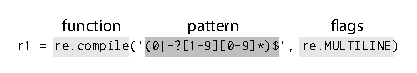
\includegraphics[width=\columnwidth]{nontex/illustrations/exampleUsage.eps}
\vspace{-12pt}
\caption{Example of one regex utilization}
\vspace{-6pt}
\label{fig:exampleUsage}
\end{figure}

\noindent \textbf{Pattern}: A \emph{pattern} is extracted from a utilization, as shown in Figure~\ref{fig:exampleUsage}. In essence, it is a string, but more formally it is an ordered series of regular expression language feature tokens.  The pattern in Figure~\ref{fig:exampleUsage}  will match if it finds a zero at the end of a line, or a (possibly negative) integer at the end of a line (i.e., due to the {\tt -?} sequence denoting zero or one instance of the {\tt -}).

Note that because the vast majority of regex features are shared across most general programming languages (e.g., Java, C, C\#, or Ruby), a Python {pattern} will (almost always) behave the same when used in other languages, whereas a utilization is not universal in the same way (i.e., it may not compile in other languages, even with small modifications to function and flag names).
As an example, the {\tt re.MULTILINE} flag, or similar, is present in Python, Java, and C\#, but  the Python {\tt re.DOTALL} flag is not present in C\# though it has an equivalent flag in Java.

In this work, we primarily focus on patterns since they are cross-cutting across languages and are the primary way of specifying the matching behavior. Next, we describe the research questions, data set collection and analysis.

We consider regex language features to be tokens that specify the matching behavior of a regex pattern, for example,  the {\tt +} in {\tt ab+}.  All studied features are listed and described in Table~\ref{table:featureStats} with examples. We then map the feature coverage for four common regex support tools, brics, hampi, RE2 and Rex, and explore survey responses regarding feature usage for some of the less supported features.\\

Regular expressions (regexes) are an abstraction of keyword search that enables the identification of text using a pattern instead of an exact keyword.  For example, the pattern \verb!`ab*c'! will match strings beginning with a, followed by zero or more b's, and ending in c, such as: `ac'!, `abc', `abbc', etc.

Regexes are commonly used for parsing text using a general purpose language like Python, validating content entered into web forms using JavaScript, and searching text files for a particular pattern using tools like grep, vim or Eclipse.

Although regexes are powerful and versatile, they can be hard to understand,  maintain, and debug, resulting in tens of thousands of bug reports~\cite{Spishak:2012:TSR:2318202.2318207}.

Regular expressions are used frequently by developers for many purposes, such as parsing files, validating user input, or querying a database.
Regexes are also employed in MySQL injection prevention~\cite{Yeole:2011:ADT:1980022.1980229} and network intrusion detection~\cite{network}.
However, recent research has suggested that regular expressions (regexes) are hard to understand, hard to compose, and error prone~\cite{Spishak:2012:TSR:2318202.2318207}.
Given the difficulties with working with regular expressions and how often they appear in software projects and processes, it seems fitting that efforts should be made to ease the burden on developers.

Our goal was to collect regexes from a variety of projects to represent the breadth of how developers use the language features.
Using the GitHub API, we scraped \dbfetch{nProjScanned} projects containing Python code.
We did so  by dividing a range of about 8 million repo IDs into 32 sections of equal size and scanning  for Python projects from the beginning of those segments until we ran out of memory. At that point, we felt we had enough data to do an analysis without further perfecting our mining techniques. We built the AST of each Python file in each project to find utilizations of the {\tt re} module functions. In most projects, almost all regex utilizations are present in the most recent version of a project, but to be more thorough, we also scanned up to 19 earlier versions. The number 20 was chosen to try and maximize returns on computing resources invested after observing the scanning process in many hours of trial scans.
All regex utilizations were obtained, sans duplicates. Within a project, a duplicate utilization was marked when two versions of the same file have the same function, pattern and flags.  In the end, we observed and recorded \dbfetch{nUsages} non-duplicate regex utilizations in \dbfetch{nProjScanned} projects.

In collecting the set of distinct patterns for analysis,  we ignore the \dbfetch{percentBadFlags}\%  of utilizations using flags, which can alter regex behavior.  An additional \dbfetch{percentInvalidPattern}\% of utilizations contained patterns that could not be compiled because the pattern was non-static (e.g., used some runtime variable).
The remaining \dbfetch{percentCleanUsages}\% (\dbfetch{nCleanUsages}) of the utilizations were collapsed into \dbfetch{nDistinctPatterns} distinct pattern strings.  Each of the pattern strings was pre-processed by removing Python quotes (\verb!`\\W!' becomes \verb!\\W!), unescaping escaped characters (\verb!\\W! becomes \verb!\W!) and parsing the resulting  string using an ANTLR-based, open source PCRE parser\footurl{https://github.com/bkiers/pcre-parser}.
This parser was unable to support \dbfetch{percentUnicode}\% (\dbfetch{N_UNICODE}) of the patterns due to unsupported unicode characters.  Another \dbfetch{percentAlien}\% (\dbfetch{N_ALIEN}) of the patterns used regex features that we  chose to exclude because they appeared very rarely (e.g., reference conditions).  An additional 0.1\% (16) of the patterns were excluded because they were empty or otherwise malformed so as to cause a parsing error.

The \dbfetch{nCorpus} distinct pattern strings that remain were each assigned a weight value equal to the number of distinct projects the pattern appeared in.  We  refer to this set of weighted, distinct pattern strings as the \emph{corpus}.

% \subsection{Experiment design}
Third, we investigate what features are supported by four large projects that aim to support regex usage (brics~\cite{brics}, hampi~\cite{hampi}, Rex~\cite{rex}, and RE2~\cite{re2}), and which features are not supported, but are frequently used by developers.

% \subsection{Implementation details}

We explore regex utilizations and flags used in the scraped Python projects.
Out of the \dbfetch{nProjScanned}\ projects scanned, \dbfetch{percentProjectsUsingRegex}\% (\dbfetch{nProjectsUsingRegex}) contained at least one regex utilization.  To illustrate how saturated projects are with regexes, we measure utilizations per project, files scanned per project, files contained utilizations, and  utilizations  per file, as shown in Table~\ref{table:saturation}.

Of projects containing at least one utilization, the average utilizations per project was 32 and the maximum  was 1,427.  The project with the most utilizations is a C\# project\footurl{https://github.com/Ouroboros/Arianrhod} that maintains a collection of source code for 20 Python libraries, including larger libraries like {\tt pip}, {\tt celery} and {\tt ipython}.  These larger Python libraries contain many utilizations.
From Table~\ref{table:saturation}, we also see that each project had an average of 11 files containing any utilization, and each of these files had an average of 2 utilizations.

\begin{figure}[tb]
\centering
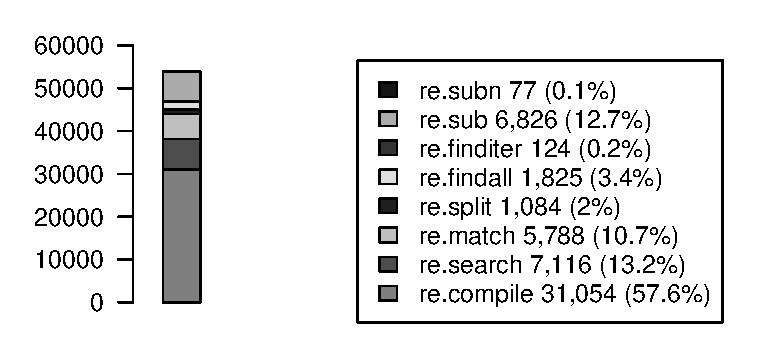
\includegraphics[width=\columnwidth]{nontex/illustrations/partFunctions.eps}
\vspace{-12pt}
\caption{How often are  {\tt re} functions used?}
\vspace{-6pt}
\label{fig:partFunctions}
\end{figure}

\begin{figure}[tb]
\centering
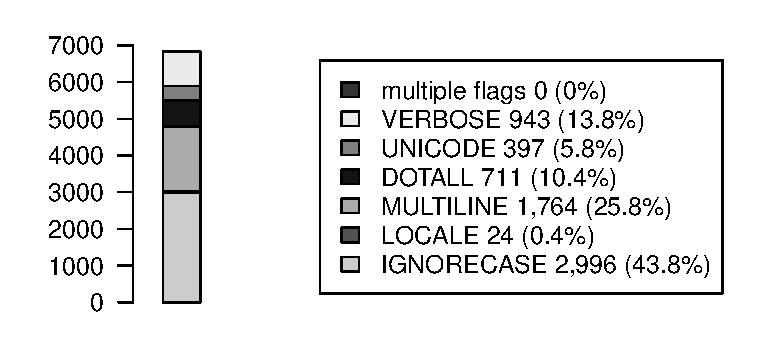
\includegraphics[width=0.9\columnwidth]{nontex/illustrations/partFlags.eps}
\vspace{-6pt}
\caption{Which behavioral flags are used?}
\vspace{-6pt}
\label{fig:partFlags}
\end{figure}


